
\chapter{jj}
\section{باب الف}
\begin{equation}
y=x
\end{equation}
\begin{equation}\label{مساوات_الف}
z=m
\end{equation}
کیا حال ہے مساوات\حوالہ{مساوات_الف}۔

\section{دوم}

\begin{figure}
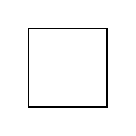
\begin{tikzpicture}
\draw(0,0) rectangle ++(1,1);
\end{tikzpicture}
\caption{شکل}
\label{شکل_الف}
\end{figure}

\begin{figure}
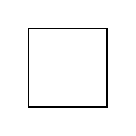
\begin{tikzpicture}
\draw(0,0) rectangle ++(1,1);
\end{tikzpicture}
\caption{شکل}
\label{شکل_دوم}
\end{figure}
شکل  \حوالہ{شکل_دوم} دیکھیں

\textup{کیا حال ہے}

\textit{کیا حال ہے}

\textsl{کیا حال ہے}

\textbf{کیا حال ہے}

\textbf{\textsl{کیا حال ہے}}


